\documentclass[11pt]{exam}
\usepackage[utf8]{inputenc}
\usepackage[T1]{fontenc}
\usepackage{amsmath, amssymb, amsopn, color, tikz}
\usepackage[margin=1in]{geometry}
\usepackage{titlesec}
\usepackage{tipa}
\usepackage{hyperref}



% Style
\setlength\parindent{0pt}
\shadedsolutions

% Define course info
\def\semester{2019-2020}
\def\course{Modèles Aléatoires Discrets M1}
\def\name{P.-O. Goffard \& Rémy Poudevigne}
%\def\quizdate{10/5, 10/6}
\def\hwknum{}
%\def\title{\MakeUppercase{Homework \hwknum -- quiz \quizdate }}
\def\title{\MakeUppercase{TD 2: Chaine de Markov}}

% Define commands
\def\Bin{\operatorname{Bin}}
\def\Geom{\operatorname{Geom}}
\def\Pois{\operatorname{Pois}}
\def\Exp{\operatorname{Exp}}
\newcommand{\E}{\mathbb E}            % blackboard E
\newcommand{\bP}{\mathbb P}            % blackboard P
\newcommand{\Var}{\text{Var}}            % blackboard P
\newcommand{\Om}{\Omega}            % blackboard P
\newcommand{\om}{\omega}            % blackboard P
\newcommand{\N}{\mathbb N}            % blackboard P
\newcommand{\R}{\mathbb R}            % blackboard P
\newcommand{\A}{\mathcal A}            % blackboard P
\def \si {\sigma}
\def \la {\lambda}
\def \al {\alpha}
% \def\e*{\end{eqnarray*}}
\def \di{\displaystyle}

\def \E{\mathbb E}
\def \N{\mathbb N}
\def \Z{\mathbb Z}
\def \NZ{\mathbb{N}_0}
\def \I{\mathbb I}
\def \w{\widehat}
\def \P {\mathbb P}
\def \V{\mathbb V}


\newcommand{\CL}{\mathbb{C}}
\newcommand{\RL}{\mathbb{R}}
\newcommand{\nat}{{\mathbb N}}
\newcommand{\Laplace}{\mathscr{L}}
\newcommand{\e}{\mathrm{e}}
\newcommand{\ve}{\bm{\mathrm{e}}} % vector e

\renewcommand{\L}{\mathcal{L}} % e.g. L^2 loss.

\newcommand{\ih}{\mathrm{i}}
\newcommand{\oh}{{\mathrm{o}}}
\newcommand{\Oh}{{\mathcal{O}}}


\newcommand{\Norm}{\mathcal{N}}
\newcommand{\LN}{\mathcal{LN}}
\newcommand{\SLN}{\mathcal{SLN}}

\renewcommand{\Pr}{\mathbb{P}}
\newcommand{\Ind}{\mathbb I}
\newcommand\bfsigma{\bm{\sigma}}
\newcommand\bfSigma{\bm{\Sigma}}
\newcommand\bfLambda{\bm{\Lambda}}
\newcommand{\stimes}{{\times}}
\def \limsup{\underset{n\rightarrow+\infty}{\overline{\lim}}}
\def \liminf{\underset{n\rightarrow+\infty}{\underline{\lim}}}
\def\euro{\mbox{\raisebox{.25ex}{{\it =}}\hspace{-.5em}{\sf C}}}
  \everymath{\displaystyle}
% \newcommand{\limsup}{\overline{\lim}\,}            % blackboard P
% \newcommand{\liminf}{\underline{\lim}\,}            % blackboard P

\begin{document}

% Heading
{\center \textsc{\Large\title}\\
	\vspace*{1em}
	\course -- \semester\\
	\name\\
	\vspace*{2em}
	\hrule
\vspace*{2em}}
\begin{questions}


\question Soit $(X_n)_{n\geq0}$ une chaîne de Markov de matrice de transition $Q$.
\begin{parts}
\part Rappeler la définition de l'irréductibilité.
\begin{solution}
Une chaîne de Markov est irréductible si tous ses états communiquent.
\end{solution}
\part Donner un exemple où $(X_n)_{n\geq0}$ n'est pas irréductible.
\begin{solution}
Un exemple de chaîne de Markov non irréductible est donné par le graphe suivant:
\[
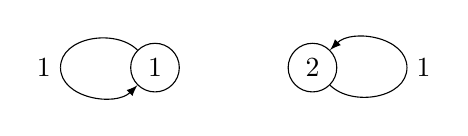
\begin{tikzpicture}
\node[draw,circle] (1)at(-1,0){1};
\node[draw,circle] (2)at(1,0){2};
\draw[-,>=latex] (1) to[out=135,in=90] (-2.2,0)node[left]{$1$};
\draw[->,>=latex] (-2.2,0)node{} to[out=-90,in=225] (1);
\draw[-,>=latex] (2) to[out=-45,in=-90] (2.2,0)node[right]{$1$};
\draw[->,>=latex] (2.2,0)node{} to[out=90,in=45] (2);
\end{tikzpicture}
\]
\end{solution}
\part Donner un exemple où il existe $i \neq j$ tels que $Q_{i,j}=0$ et la chaîne est irréductible.
\begin{solution}
Dans l'exemple suivant, $Q_{1,3}=0$ mais la chaîne est irréductible :
\[
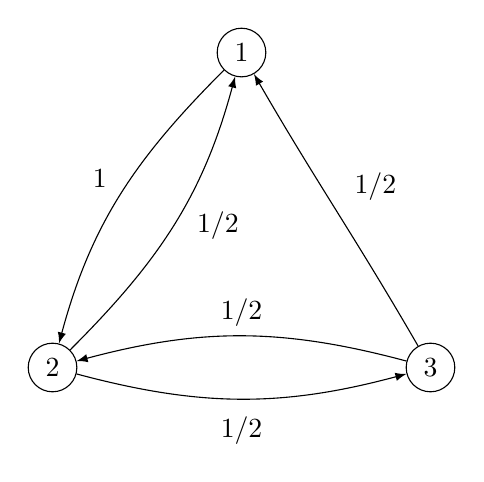
\begin{tikzpicture}
\node[draw,circle] (1)at(0,4){1};
\node[draw,circle] (2)at(-2.4,0){2};
\node[draw,circle] (3)at(2.4,0){3};
\draw[->,>=latex] (1) to[out=225,in=75] (2);
\draw[->,>=latex] (2) to[out=45,in=255] (1);
\draw[->,>=latex] (2) to[out=-15,in=195] (3);
\draw[->,>=latex] (3) to[out=120,in=-60] (1);
\draw[->,>=latex] (3) to[out=165,in=15] (2);
\node at(-1.8,2.4) {$1$};
\node at(-0.3,1.8) {$1/2$};
\node at(0,-0.8) {$1/2$};
\node at(0,0.7) {$1/2$};
\node at(1.7,2.3) {$1/2$};
\end{tikzpicture}
\]
\end{solution}
\part Soit $N\geq0$ fixé. Donner un exemple où il existe $i, j$ tels que pour tout $k\leq N$, $(Q^k)_{i,j}=0$ mais la chaîne est irréductible.
\begin{solution}
Pour la chaîne de Markov donnée par le graphe suivant, on a que pour tout $k\leq N$, $(Q^k)_{1,N+2}=0$ :
\[
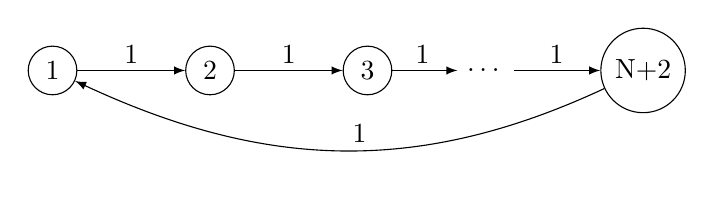
\begin{tikzpicture}
\node[draw,circle] (1)at(-1,0){1};
\node[draw,circle] (2)at(1,0){2};
\node[draw,circle] (3)at(3,0){3};
\node (4)at(4.5,0){$\dots$};
\node[draw,circle] (5)at(6.5,0){N+2};
\draw[->,>=latex] (1) to (2);
\draw[->,>=latex] (2) to (3);
\draw[->,>=latex] (3) to (4);
\draw[->,>=latex] (4) to (5);
\draw[->,>=latex] (5) to[out=-155,in=-25] (1);
\node at(0,0.2){1};
\node at(2,0.2){1};
\node at(3.7,0.2){1};
\node at(5.4,0.2){1};
\node at(2.9,-0.8){1};
\end{tikzpicture}
\]
\end{solution}
\end{parts}

\question \textbf{Maladie contagieuse} \\
Une maladie s'attrape avec une probabilité $0,05$. Quand on l'a attrapée on peut soit en guérir soit acquérir des séquelles irréversibles. Ces séquelles sont associées à une immunité totale par la suite. Si on guérit, en revanche, on n'est immunisé que dans $50\%$ des cas. Dans la population, par ailleurs, $1$ personne sur $5$ est naturellement immunisée.
\begin{parts}
\part Modéliser l'état d'un individu dans la période de temps $(n, n + 1)$ par une chaîne de Markov. Donner son graphe, sa loi initiale et sa matrice de transition.
\begin{solution}
On peut modéliser la chaîne de Markov par $4$ états :
\begin{itemize}
\item sain (S),
\item malade (M),
\item immunisé sans séquelles (I),
\item immunisé avec séquelles (IS).
\end{itemize}
On obtient le graphe suivant, où $p_G$ est la probabilité de guérir sans séquelles :
\[
\begin{tikzpicture}
\node[draw,circle] (1)at(2,2){M};
\node[draw,circle] (2)at(-2,2){S};
\node[draw,circle] (3)at(-2,-2){I};
\node[draw,circle] (4)at(2,-2){IS};
\draw[->,>=latex] (1) to[out=-160,in=-30] (2);
\draw[->,>=latex] (2) to[out=30,in=160] (1);
\draw[->,>=latex] (1) to (3);
\draw[->,>=latex] (1) to (4);
\draw[-,>=latex] (2) to[out=155,in=90] (-4.0,2)node[left]{$0,95$};
\draw[->,>=latex] (-4.0,2)node{} to[out=-90,in=205] (2);
\draw[-,>=latex] (3) to[out=200,in=135] (-3.6,-3.4)node[left]{1};
\draw[->,>=latex] (-3.6,-3.4)node{} to[out=-45,in=250] (3);
\draw[-,>=latex] (4) to[out=-20,in=45] (3.6,-3.4)node[right]{1};
\draw[->,>=latex] (3.6,-3.4)node{} to[out=225,in=-70] (4);
\node at(0.2,-0.6){$\frac{p_G}{2}$};
\node at(2.5,0){$1\!-p_G$};
\node at(-0.1,1.0){$\frac{p_G}{2}$};
\node at(-0.1,2.8){0.05};
\end{tikzpicture}
\]
La matrice de transition correspondante est donc :
\[
\left(\begin{matrix}
0,95 & 0,05 &0 &0 \\[4pt]
\frac{p_G}{2} & 0 &\frac{p_G}{2} &1-p_G \\[6pt]
0 & 0 &1 &0 \\
0 & 0 &0 &1 
\end{matrix}\right)
\]
\end{solution}
\part Classifier les états.
\begin{solution}
L'état $I$ ne communique avec aucun état et il est récurrent.\\
L'état $IS$ ne communique avec aucun état et il est récurrent.\\
Si $p_G>0$, les états $S$ et $M$ communiquent et forment une classe d'équivalence transitoire.\\
Si $p_G=0$, $S$ ne communique avec aucun état et il est transitoire et $M$ ne communique avec aucun état et il est transitoire.
\end{solution}
\part Quelle est la probabilité qu'une personne attrape la maladie 2 fois de suite et s'en sorte sans séquelle mais non immunisée ?
\begin{solution}
On considère qu'à l'instant $0$, une personne est dans l'état $I$ avec probabilité $1/5$ et dans l'état $S$ avec probabilité $4/5$. La probabilité d'être malade 2 fois de suite et de s'en sortir dans séquelle mais non immunisé est donc égale à :
\[
\begin{aligned}
&\P(X_0=S,X_1=M,X_2=S,X_3=M,X_4=S)\\
=&\P(X_0=S)\P(X_1=M|X_0=S)\P(X_2=S|X_1=M)\P(X_3=M|X_2=S)\P(X_4=S|X_3=M)\\
=&\frac{4}{5}0.05\frac{p_G}{2}0.05\frac{p_G}{2}\\
=&\frac{p_G^2}{1000}.
\end{aligned}
\]
\end{solution}
\part Existe-t-il une probabilité invariante ? Est-elle unique ? Pourquoi ?
\begin{solution}
On a une chaîne de Markov sur un nombre fini d'états, il y a donc au moins une mesure invariante. Il n'y a cependant pas unicité de la mesure invariante puisque pour tout $x\in[0,1]$, la mesure $\mu_x$ définie par :
\[
\mu_x(\{I\})=x \text{ et } \mu_x(\{IS\})=1-x
\]
est invariante.
\end{solution}
\end{parts}


\question { \bf Jeu de soccer}\\
Le soccer se joue à $2$ équipes, composées chacune de $10$ joueurs et $1$ goal. Chaque équipe se partage sur le terrain en $3$ zones : défense-centre-attaque (ex: une configuration $3-4-4$ correspond à $3$ défenseurs, $4$ milieu et $4$ attaquants). On supposera que tous les joueurs sont de niveau équivalent.\\
On regarde la position de la balle, qui ne peut être qu'à $5$ endroits : but de gauche, défense gauche, milieu, défense droite ou but de droite. A chaque instant, la balle doit aller à droite ou à gauche, et les chances sont proportionnelles au nombre de joueurs dans la zone, selon la configuration des équipes. Lorsque la balle atteint un but, elle retourne au milieu à l'instant suivant, et un but est marqué.
\begin{parts}
\part Supposons que l'équipe $A$ adopte la configuration $3-4-4$ et l'équipe $B$ la configuration $5-3-3$
\begin{itemize}
\item[(i)] Modéliser ce problème avec une chaîne de Markov homogène. Quelle est sa mesure initiale, sa matrice de transition ?
\item[(ii)] La chaîne est-elle irréductible? Calculer la mesure de probabilité invariante.
\item[(iii)] Sous la mesure de probabilité invariante, quelle est la probabilité moyenne de toucher le but $A$ ? le but $B$ ? Quelle est la meilleure stratégie ?
\item[(iv)] On considère que la balle change de zone $3$ fois par minute, et que le jeu dure $60$ minutes. Donner une approximation du score moyen.
\end{itemize}
\begin{solution}
\begin{enumerate}
\item On modélise l'état de la balle à l'instant $n$ par une
chaîne de Markov homogène à $5$ états. Cette chaîne est
irréductible (tous les états communiquent). La chaîne est donnée par le graphe suivant :\\
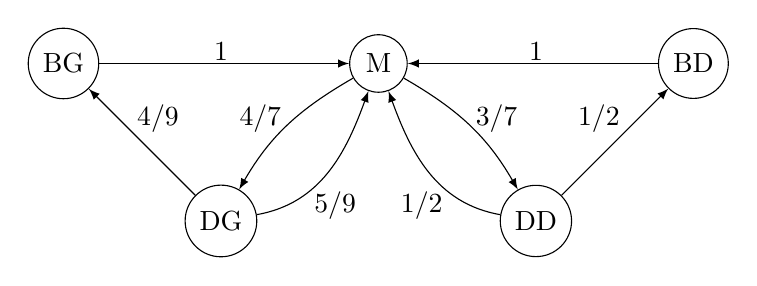
\begin{tikzpicture}
\node[draw,circle] (BG)at(-4,1){BG};
\node[draw,circle] (DG)at(-2,-1){DG};
\node[draw,circle] (M)at(0,1){M};
\node[draw,circle] (DD)at(2,-1){DD};
\node[draw,circle] (BD)at(4,1){BD};
\draw[->,>=latex] (BG) to (M);
\draw[->,>=latex] (DG) to (BG);
\draw[->,>=latex] (DG) to[out=10,in=-110] (M);
\draw[->,>=latex] (M) to[out=210,in=60] (DG);
\draw[->,>=latex] (BD) to (M);
\draw[->,>=latex] (DD) to[out=170,in=-70] (M);
\draw[->,>=latex] (M) to[out=-30,in=120] (DD);
\draw[->,>=latex] (DD) to (BD);
\node at(-2,1.15) {$1$};
\node at(2,1.15) {$1$};
\node at(-2.8,0.3) {4/9};
\node at(-1.5,0.3) {4/7};
\node at(1.5,0.3) {3/7};
\node at(2.8,0.3) {1/2};
\node at(-0.55,-0.8) {5/9};
\node at(0.55,-0.8) {1/2};
\end{tikzpicture}\\
La mesure initiale est $\mu_0=\delta_M$ puisque le ballon part du
milieu du terrain. La matrice de transition est la suivante :
$$ P=\left( \begin{array}{ccccc}
0 & 0 & 1 & 0 & 0  \\
4/9 & 0 & 5/9 & 0 & 0 \\
0 & 4/7 & 0 & 3/7 & 0 \\
0 & 0 & 1/2 & 0 & 1/2 \\
0 & 0 & 1 & 0 & 0 \\
\end{array} \right)
$$
\item Le comportement de la balle à long terme correspond à la
probabilité de la balle d'être dans les différents états "à long
terme", c'est-à-dire lorsque l'on se place en régime stationnaire
: c'est ce que représente la mesure invariante. Or ici on a une
chaîne de Markov irréductible sur un espace d'états fini, donc il
y a une unique mesure stationnaire. On la calcule en résolvant
l'équation $\mu P=\mu$, avec $\sum_i \mu_i = 1$. Cela nous donne
le système suivant :
$$
\left\{
\begin{array}{c}
4/9\mu_2=\mu_1 \\
4/7\mu_3=\mu_2 \\
\mu_1+5/9\mu_2+1/2\mu_4+\mu_5=\mu_3 \\
3/7\mu_3=\mu_4 \\
1/2\mu_4=\mu_5 \\
\mu_1+\mu_2+\mu_3+\mu_4+\mu_5=1
\end{array}\right.
\Rightarrow \left\{ \begin{array}{c}
\mu_1= 32/311\\
\mu_2=72/311 \\
\mu_3=126/311 \\
\mu_4=54/311 \\
\mu_5=27/311 \\
\end{array}
\right.$$ \item La probabilité moyenne de toucher le but $A$ (ou
le $B$) correspond donc à la probabilité d'être en $BD$ en régime
stationnaire, donc P(toucher but A)=$\mu_5=27/311$ et P(toucher
but B)=$\mu_1=32/311$. Donc on a plus de chances de marquer dans
le but $B$, et donc la stratégie de $A$ est la meilleure : $3-4-4
> 5-3-3$.


\item On considère que la balle change de zone $3$ fois par
minute, et que le jeu dure $60$ minutes. Le score moyen de
l'équipe $B$ correspond au nombre de buts marqués dans le but $A$,
soit $60 \times 3 \times \mu_5 \cong 15$ et celui de l'équipe $A$ est
$60 \times 3\times \mu_1\cong 18$. Donc score moyen $A-B$ :
$18-15$. La stratégie de $A$ est donc la meilleure.
\end{enumerate}

\end{solution}
\part Comparaison de stratégies
\begin{itemize}
\item[(i)] Comparer les stratégies $3-4-4$ et $4-4-3$.
\item[(ii)] Comparer les stratégies $5-3-3$, $3-4-4$ et $4-3-4$.
\end{itemize}
\begin{solution}
\begin{enumerate}
\item Une étude similaire avec les stratégies $3-4-4$ et $4-4-3$
nous donnent la matrice suivante :
$$ P=\left( \begin{array}{ccccc}
0 & 0 & 1 & 0 & 0  \\
1/2 & 0 & 1/2 & 0 & 0 \\
0 & 1/2 & 0 & 1/2 & 0 \\
0 & 0 & 1/2 & 0 & 1/2 \\
0 & 0 & 1 & 0 & 0 \\
\end{array} \right)
$$
On obtient pour la mesure stationnaire :
$\mu_1=\mu_5=\frac{1}{10}$, $\mu_2=\mu_4=\frac{1}{5}$ et
$\mu_3=\frac{2}{5}$. On a un jeu équitable, ou équilibré : les
stratégies $A$ et $B$ se valent, la probabilité de marquer en $A$
est la même qu'en $B$.

\item De la même manière, on peut comparer et trouver que la
stratégie $3-4-4$ est meilleure que la $4-3-4$ et que la $5-3-3$,
ce qui est compatible avec le fait que $3-4-4$ était meilleure que
$5-3-3$. En revanche, on peut trouver des stratégies qui sont
comparables 2 à deux mais qui ne sont pas ordonnables en
globalité. Par exemple, $5-2-4 > 4-3-4$ et $4-3-4 > 5-3-3$ mais
$5-3-3 > 5-2-4$. En effet, l'ordre que l'on vient d'établir entre
les stratégies n'est pas total : il n'y a pas de stratégie
gagnante à tous les coups.
\end{enumerate}
\end{solution}
\end{parts}

\end{questions}
\end{document}
